%!TEX program = lualatex
% aspect ratio: 16:9
\documentclass[unicode, 9pt, aspectratio=169]{beamer}
\usepackage{mybeamer}
\usepackage{luatexja-otf}
\usepackage[]{graphicx}
\usepackage{amsmath}


\title{ROSを用いた遠隔型自動運転システムの開発}
\author{ME2208 \CID{8705}橋 尚太郎\\指導教員  野村 隼人}
\institute{明石工業高等専門学校 専攻科 機械・電子システム工学専攻1年}
\date{2023年1月27日}


\begin{document}

\maketitle

\begin{frame}
  \frametitle{発表概要}
  \centering
    \begin{block}{}
      \begin{enumerate}
        \item はじめに
        \item 実証事例
        \item 実証実験環境の比較
        \item 提案・目標設定
        \item 実装
        \item 実験
        \item 実験結果
        \item 考察・結論
        \item おわりに
      \end{enumerate}
    \end{block}
\end{frame}

\begin{frame}
  \frametitle{はじめに}
  $\blacksquare$ 自動運転は地方交通での需要があり既に実現・実用化されている
  \begin{center}
    \begin{minipage}{.8\linewidth}
        \begin{block}{}
            \centering
            \begin{tabular}{ccc}
                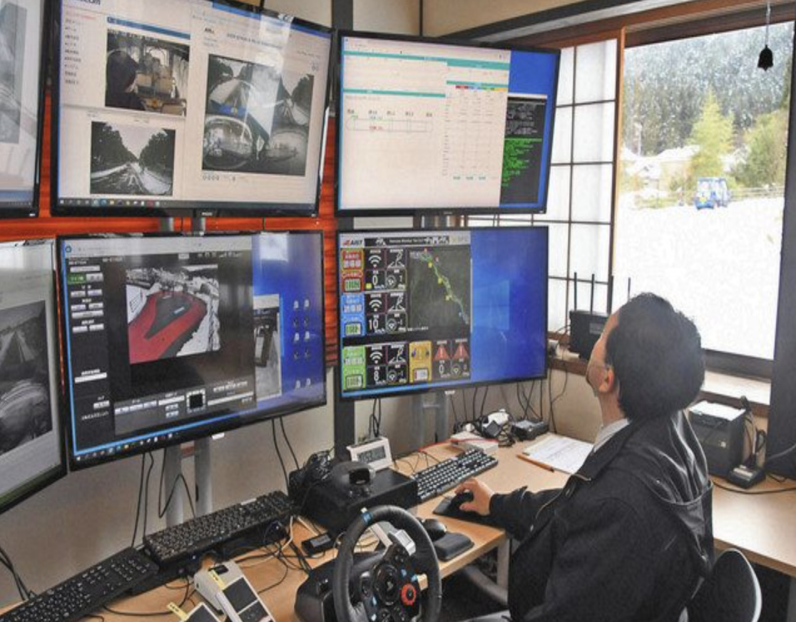
\includegraphics[height=.4\textheight]{img/jikken3.pdf}
                &
                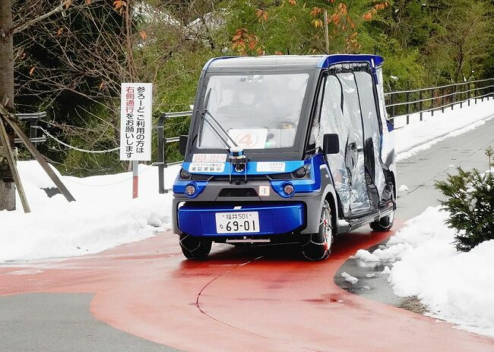
\includegraphics[height=.4\textheight]{img/jikken4.pdf}
                \\ \tiny モニターを見ながら自動走行車（右奥）を遠隔監視するスタッフ & \tiny 自動運転「ZEN drive」,福井県永平寺町\\
            \end{tabular}
            \\{\tiny [参考] 永平寺町の自動走行車両サービス　１人で３台遠隔監視　：日刊県民福井Web \url{https://www.chunichi.co.jp/article/174299}}
        \end{block}
    \end{minipage}
\end{center}
\centering  
\Large \emph{しかし法律の面で運用に制限がある(実証段階にとどまっている)}\\
  \centering
  \begin{minipage}{.5\linewidth}
    \begin{alertblock}{}
        \centering
        \Large \emph{法制度に合わせた実証実験の仕組みが必要}
    \end{alertblock}
  \end{minipage}
\end{frame}

\begin{frame}
  \frametitle{実証事例}
  $\blacksquare$ 実証実験の仕組み\\
  \hrulefill\\
  \centering
  \begin{minipage}{.5\linewidth}
    \begin{exampleblock}{}
        \centering
        \Large \emph{公道での実証実験には法定基準がある}
    \end{exampleblock}
  \end{minipage}

  \begin{description}
    \item[ex.] 遠隔型自動運転に関する実証実験\\
  $\to$ 現行の法律では遠隔監視者(自動運転の異常時に対応するための人)との\textbf{\textcolor{red}{複数人管理}}が\underline{必要}
    \item[遠隔監視者] \textbf{\textcolor{red}{運転免許}}$+$\textbf{\textcolor{red}{法定の訓練}}が\underline{必要} (運転免許の所持が義務)
  \end{description}
  \begin{figure}
    \begin{minipage}{.8\linewidth}
      \centering
      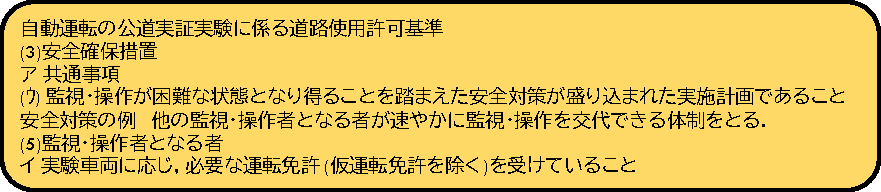
\includegraphics[width=.8\textwidth]{img/houritsu.pdf}
    \end{minipage}
  \end{figure}
  \hrulefill\\
  \centering
  \begin{minipage}{.5\linewidth}
    \begin{alertblock}{}
        \centering
        \Large \emph{\textcolor{red}{これらは全て実車を用いた実証実験環境}}
    \end{alertblock}
  \end{minipage}
\end{frame}

\begin{frame}
  \frametitle{実証実験環境の比較}
  \begin{center}
        \begin{block}{}
          \begin{figure}
            \begin{minipage}{.8\linewidth}
              \centering
              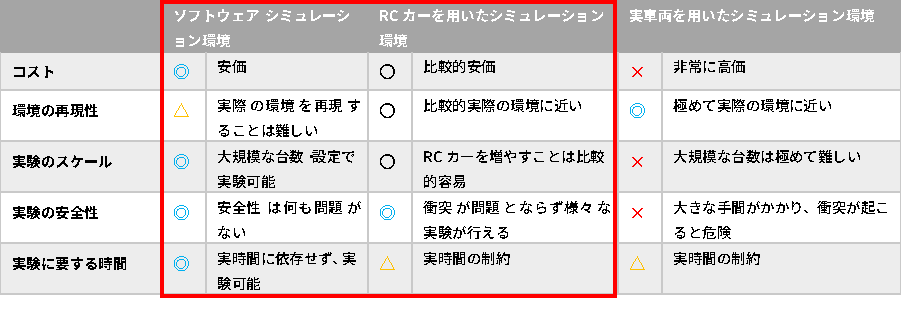
\includegraphics[width=\textwidth]{img/hyou.pdf}
            \end{minipage}
          \end{figure}
        \end{block}
\end{center}
\centering
\begin{minipage}{.8\linewidth}
\centering
\vspace{-3.5truemm}
\begin{exampleblock}{ソフトウェアシミュレーションとRCカーの併用が妥当}
  実時間に依存しない検証・評価 $\to$ ソフトウェアシミュレーション環境\\
  再現性の必要な検証・評価 $\to$ RCカーを用いた操作環境\\
\end{exampleblock}
\vspace{-2.5truemm}
  \begin{alertblock}{}
    \centering
    \Large \emph{\textcolor{red}{運転免許の有無に依存しない操作環境という枠組みを確立}}
  \end{alertblock}
\end{minipage}

\end{frame}

\begin{frame}
  \frametitle{提案・目標設定}
  \centering
  \begin{minipage}{.8\linewidth}
    \begin{block}{課題}
      自動運転の実証に向けた法整備が進んでいないことで運用に制限がある\\
      \centering
      \Large \emph{\textcolor{red}{法定の訓練が必要でない環境があると自動運転の研究/実証が手軽に}}
    \end{block}

    \begin{alertblock}{目標設定}
      \begin{description}[目的]
        \item[目的] 運転免許の所持不所持に関わらず遠隔型自動運転の実験に携わることが可能な\\練習および研究のための環境構築
        \item[提案] \textcolor{red}{ROSを用いた遠隔型自動運転システム}
        \item[方法] インターフェースの操作性に基づく運転技能解析の追究
        \\ \textcolor{red}{AT・MT・セミAT}インターフェースによる遠隔型自動運転環境の構築
      \end{description}
    \end{alertblock}
  \end{minipage}

  \begin{minipage}{.6\linewidth}
      \begin{exampleblock}{}
          \centering
          \Large \emph{キーワード}
      \end{exampleblock}
      \begin{itemize}
        \item[＊]遠隔型自動運転、操作性、ヒューマンマシンインターフェース  
      \end{itemize}
  \end{minipage}
\end{frame}

\begin{frame}
  \frametitle{実装}
  \centering
  \begin{minipage}{.8\linewidth}
  \begin{exampleblock}{作成した遠隔型自動運転環境の満たすべき条件}
    \begin{itemize}
      \item 運転免許を所持していなくても\textbf{実機}でのインタラクションが可能
      \item 乗用車における多様なマシンインターフェースで操作が可能
    \end{itemize}
  \end{exampleblock}
\end{minipage}
  
  \begin{minipage}{.8\linewidth}
    \begin{alertblock}{解決方法}
      \begin{itemize}
        \item 走行実験により検証
        \item \textcolor{red}{RCカーにAT/MT/セミAT機能を実現} $\to$ 新規性
        \\$\to$ ROSによる実装で\textbf{遠隔操作$+$自動運転機能の実装を視野}にシステム開発
      \end{itemize}
    \end{alertblock}
  \end{minipage}
\end{frame}

\begin{frame}
  \frametitle{実験}
  \begin{description}[目的]
    \item[目的] 運転免許不所持者を含めた運転操作インタラクションの分析
    \item[方法] 走行操作の体感情報を記録、ブレーキ操作の記録\\操作に関する被験者の体感情報の記録(アンケート)
  \end{description}
  \begin{enumerate}
    \item 操作インターフェースを自由に1つ選び自由にコースを走行(AT/MT/セミAT)
    \item ブレーキテストを実施
  \end{enumerate}
  \begin{center}
    \vspace{-8pt}

    \hrulefill

    \begin{tabular}{cc}
        \begin{minipage}{.5\linewidth}
            自由走行環境
            \begin{figure}
              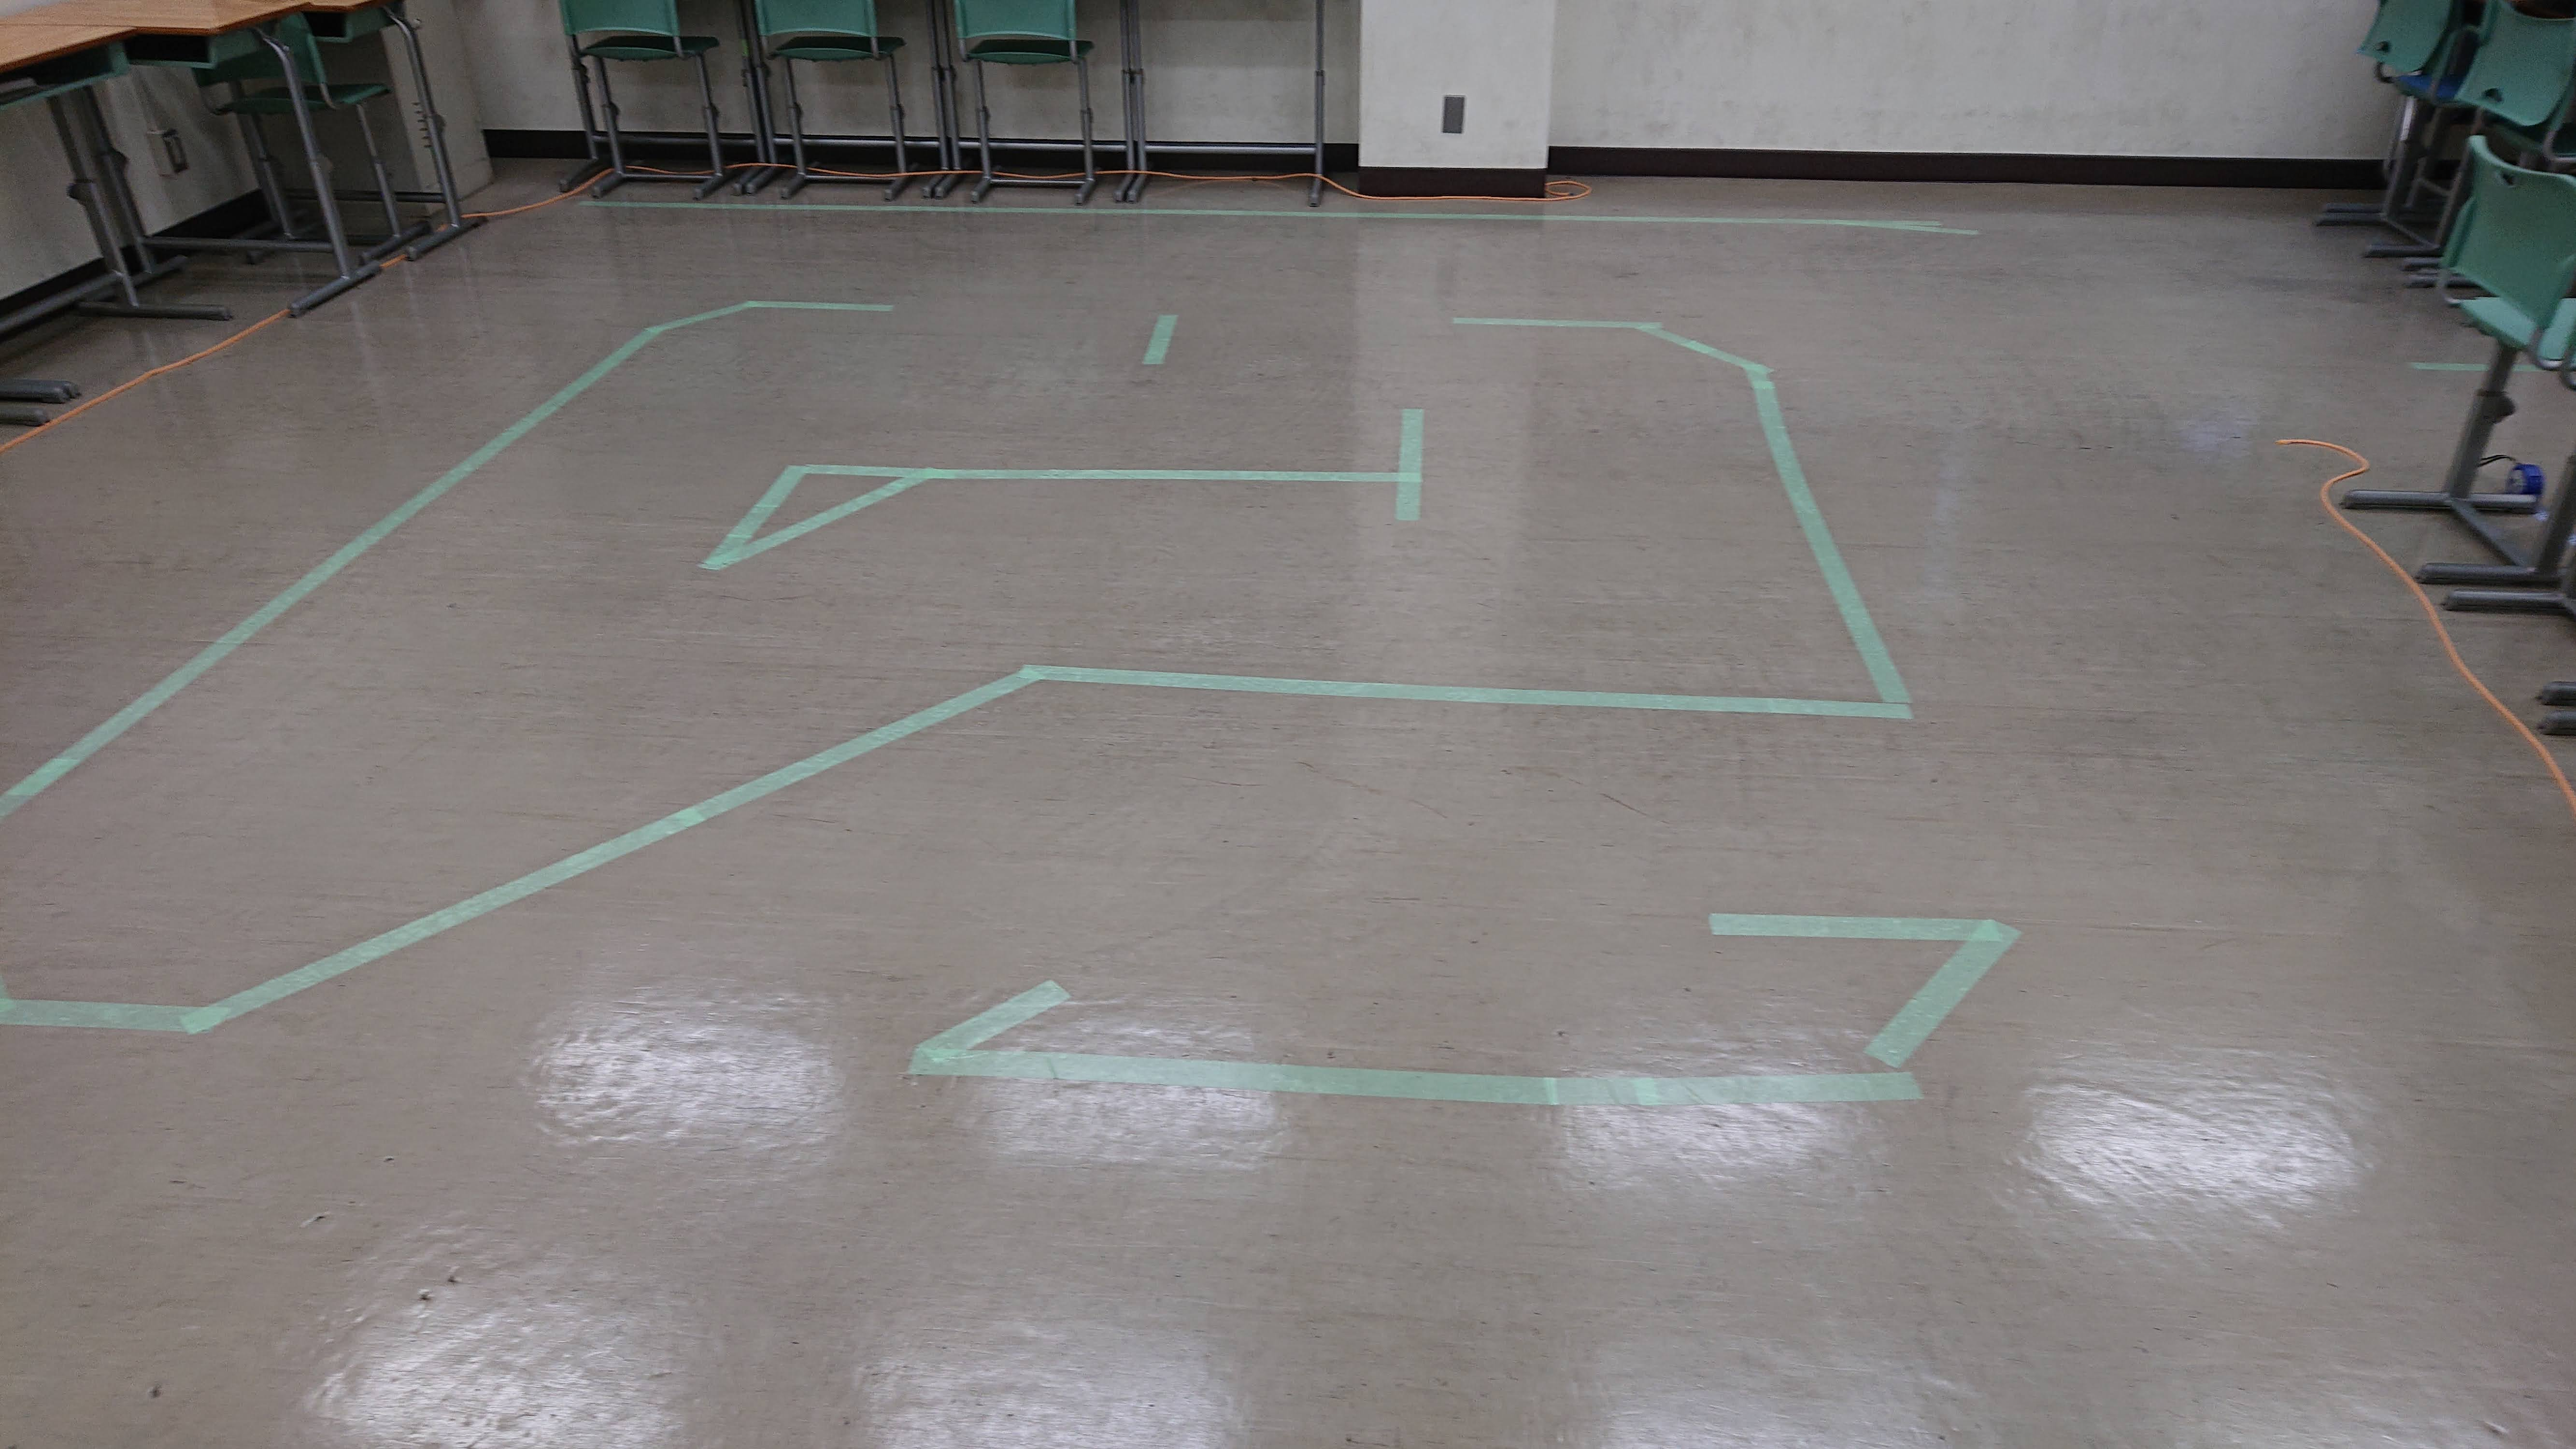
\includegraphics[width=.8\textwidth]{img/circuit.JPG}
            \end{figure}
        \end{minipage}
        &
        \begin{minipage}{.5\linewidth}
            ブレーキテスト環境
            \begin{figure}
              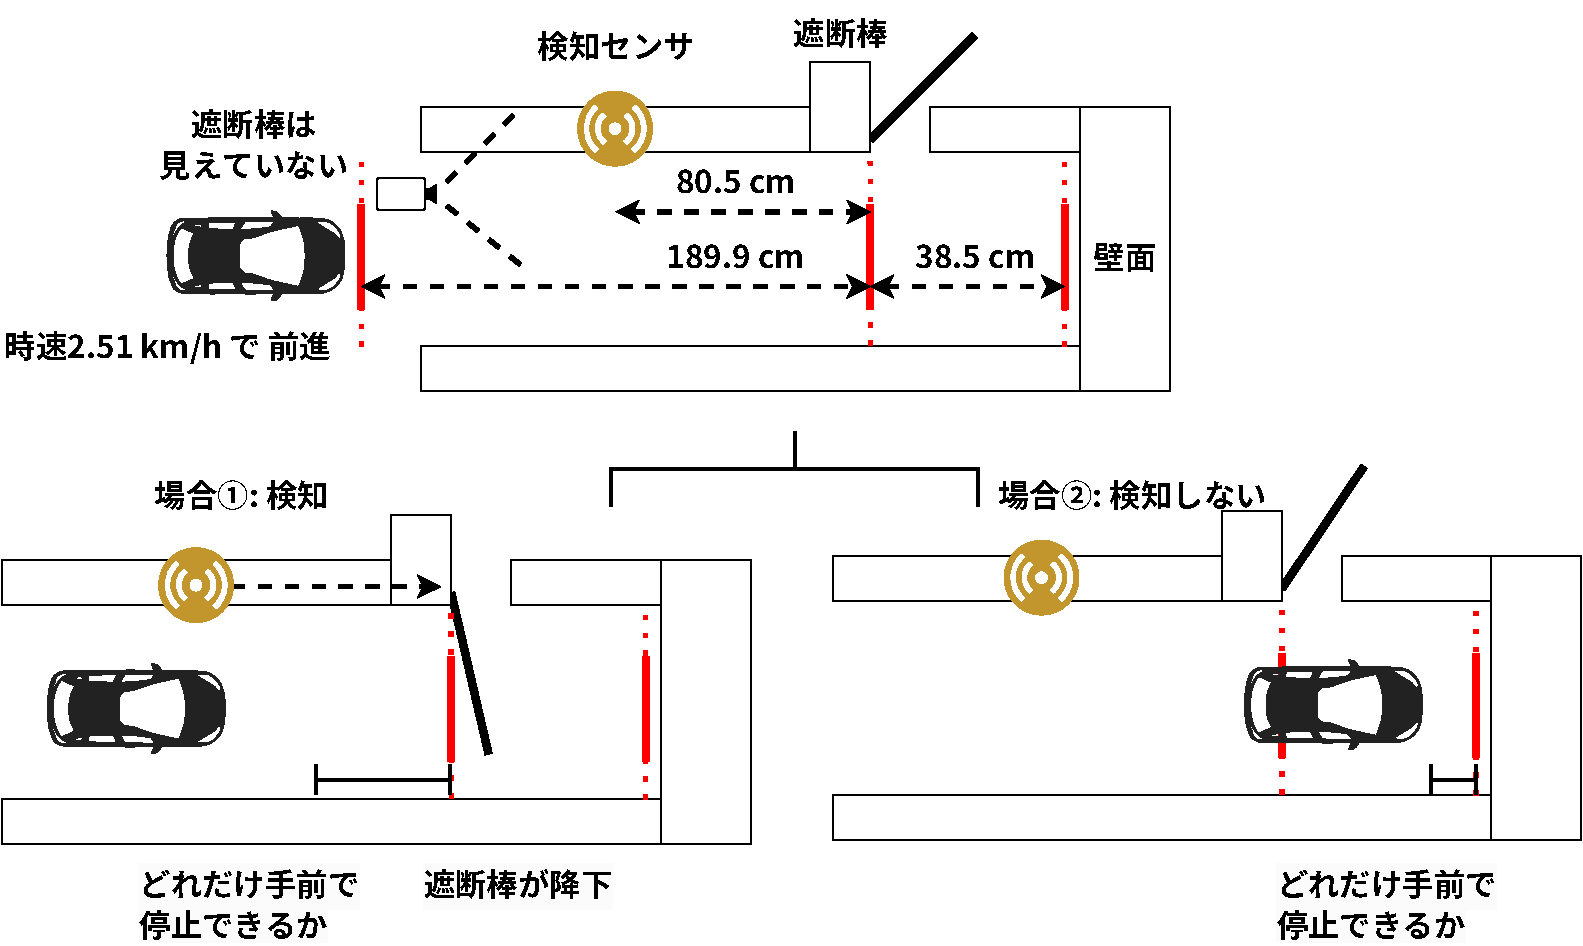
\includegraphics[width=.8\textwidth]{img/jikkenn.pdf}
            \end{figure}
        \end{minipage}
    \end{tabular}
\end{center}
\end{frame}

\begin{frame}
  \frametitle{実験結果}
  $\blacksquare$ 被験者46人がアンケートに回答\\
  $\blacksquare$ ブレーキテストは希望者のみ実施(33人)
  \begin{center}
    \vspace{-8pt}

    \hrulefill

    \begin{tabular}{cccc}
        \begin{minipage}{.22\linewidth}
            \begin{figure}
              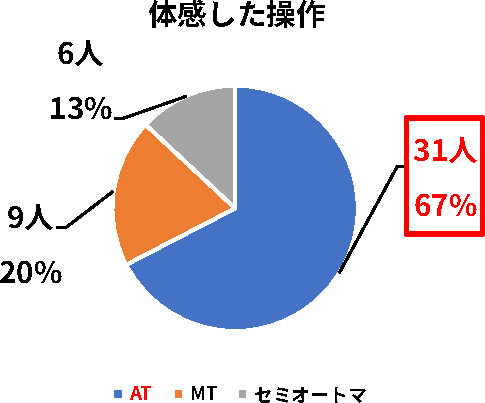
\includegraphics[width=\textwidth]{img/an1.pdf}
            \end{figure}
            \begin{figure}
              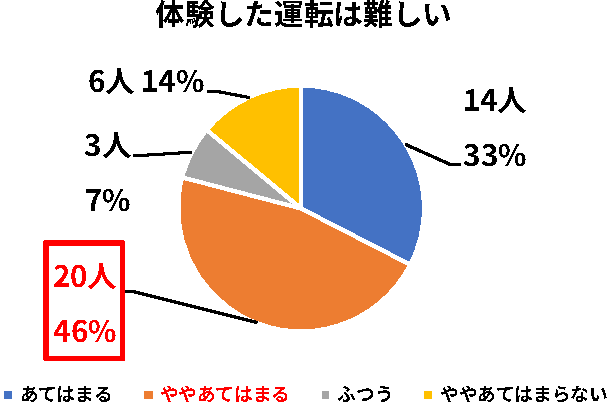
\includegraphics[width=\textwidth]{img/an5.pdf}
            \end{figure}
        \end{minipage}
        &
        \begin{minipage}{.22\linewidth}
            \begin{figure}
              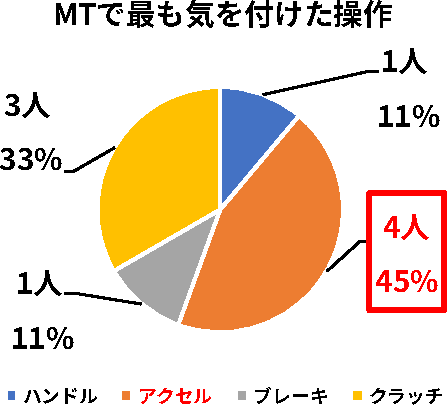
\includegraphics[width=\textwidth]{img/an2.pdf}
            \end{figure}
            \begin{figure}
              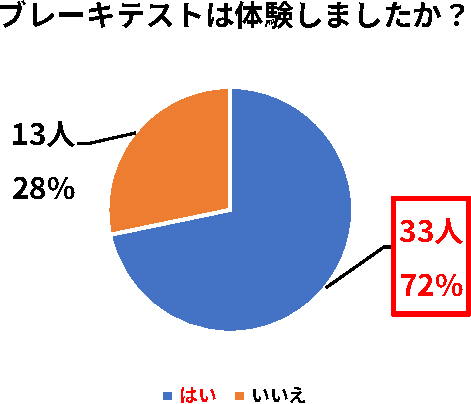
\includegraphics[width=\textwidth]{img/an6.pdf}
            \end{figure}
        \end{minipage}
        &
        \begin{minipage}{.22\linewidth}
            \begin{figure}
              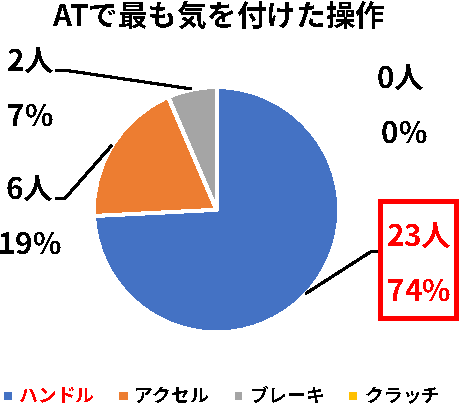
\includegraphics[width=\textwidth]{img/an3.pdf}
            \end{figure}
            \begin{figure}
              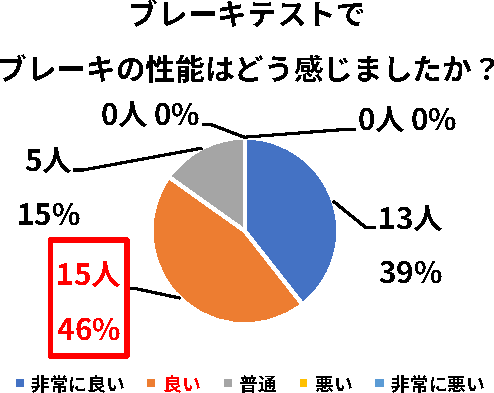
\includegraphics[width=\textwidth]{img/an7.pdf}
            \end{figure}
        \end{minipage}
        &
        \begin{minipage}{.22\linewidth}
            \begin{figure}
              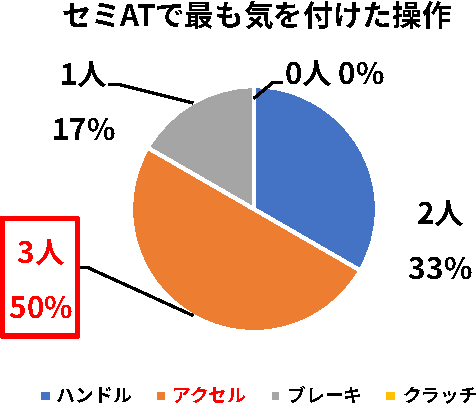
\includegraphics[width=\textwidth]{img/an4.pdf}
            \end{figure}
            \begin{figure}
              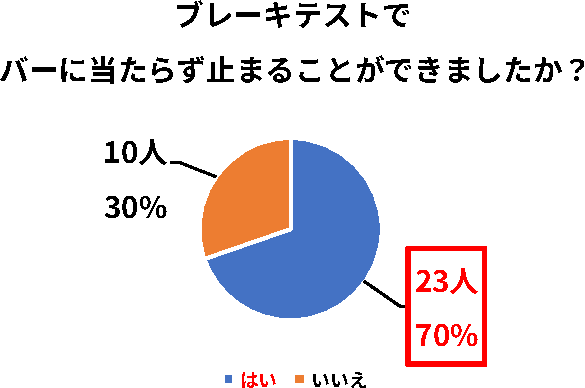
\includegraphics[width=\textwidth]{img/an8.pdf}
            \end{figure}
        \end{minipage}

    \end{tabular}
\end{center}
\end{frame}

\begin{frame}
  \frametitle{考察・結論}
  \centering
  \begin{minipage}{.8\linewidth}
  \begin{block}{考察}
    \begin{itemize}
      \item 比較的簡単なAT操作を選択する人が\textcolor{red}{67\%}、同時に\textcolor{red}{79\%}が操作を難しいと回答
      \item 若年層(未就学児~小中学生)の被験者が多い(全体の6～7割)
      \item \textcolor{red}{若年層は全員AT操作を選択 $\to$ AT操作選択者の74\%がハンドル操作に注力}
    \end{itemize}
  \end{block}
  \vspace{-3.5truemm}
  \begin{alertblock}{}
    \centering
    \Large \emph{\textcolor{red}{ハンドルの操作に慣れていないため注力}}
  \end{alertblock}
\end{minipage}
  \begin{minipage}{.8\linewidth}
    \begin{exampleblock}{若年層が難しいと感じるハンドル操作}
      \begin{itemize}
        \item カウンターステア(曲がる方向にステアを切ったあとに元に戻す操作)ができない
        \item 大人やMT/セミAT操作の選択者は難なくハンドルを操作 $\to$ \textcolor{red}{操作が実車より簡単}
      \end{itemize}
    \end{exampleblock}
  \end{minipage}
  \begin{minipage}{.8\linewidth}
    \begin{alertblock}{結論}
      \begin{center}
        \Large \emph{\textcolor{red}{若年層に向けたステアリング操作の工夫が重要}}\\
        \Large \emph{\textcolor{red}{ステアリング補正機能の実現により目的達成の方向性を検討する}}
      \end{center}
    \end{alertblock}
  \end{minipage}
\end{frame}

\begin{frame}
  \frametitle{おわりに}
  $\blacksquare$ 個々の運転技能に応じたインターフェースによって実機でのインタラクションを実現\\
  $\blacksquare$ 若年層に向けたステアリング操作の補正が必要
  $\to$ 目的達成の方向性を検討\\
  $\blacksquare$ 今後の展望
  \begin{block}{自動運転⇔手動運転の引継ぎにおける操作性}
    \begin{description}[体感速度]
      \item[研究目標] LiDARセンサ${}^\text{※}$を活用した手動/自動運転引継ぎシステムの開発
      \item[概要] 自動運転中の\textcolor{red}{運転以外の動作}が引継ぎに与える影響をシミュレーションと比較\\(ex. 携帯操作(電話・動画視聴・ゲーム・メール)、カーナビの注視)
    \end{description}
  \end{block}

  \begin{center}
    \vspace{-8pt}

    \hrulefill

    \begin{tabular}{cc}
        \begin{minipage}{.5\linewidth}
          \begin{block}{体感速度に関する研究}
            \begin{description}[体感速度]
              \item[体感速度] 実車操作$＜$本システム操作
              \item[方法] 視覚的な錯覚 → 幾何学的仮説 \textcolor{red}{体系的に追及}
            \end{description}
          \end{block}
        \end{minipage}
        &
        \begin{minipage}{.5\linewidth}
          \begin{figure}
            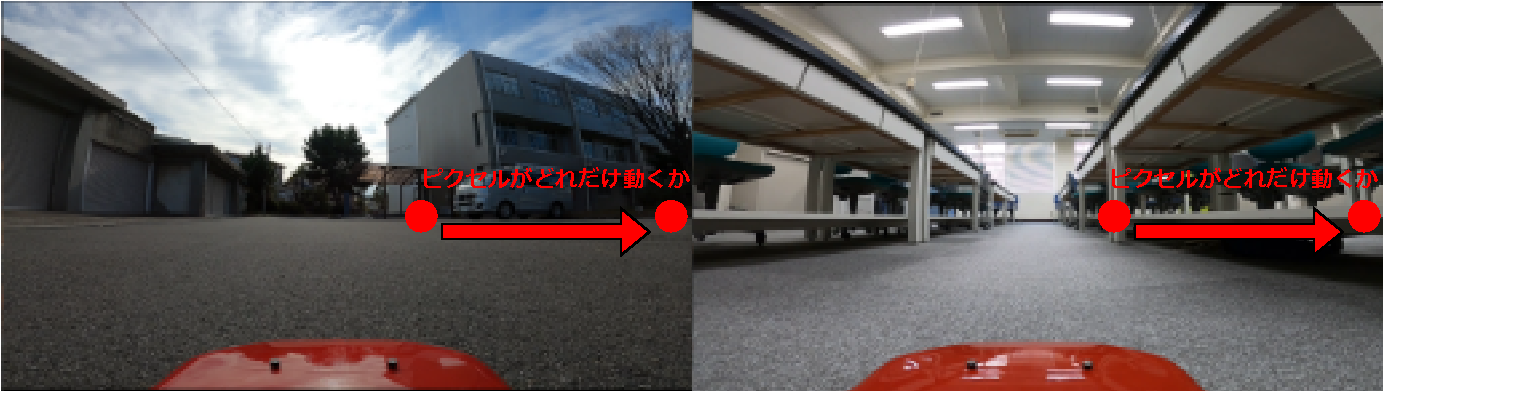
\includegraphics[width=.8\textwidth]{img/taikan_pix.pdf}
          \end{figure}
        \end{minipage}
    \end{tabular}
\end{center}
{\footnotesize [※フレッシュラボ応援プログラム] 北陽電機株式会社様よりLiDARセンサ（URG-04LX-UG01）を無償貸与}
\end{frame}

\appendix

\begin{frame}
  \frametitle{付録:自動運転のレベル分け}
  $\blacksquare$ 日本政府は2023年4月に自動運転レベル4を道路交通法で施行\\
  $\to$レベル4:過疎地等で無人の車両が遠隔監視の下で走る「無人自動運転移動サービス」を想定
  \begin{figure}
    \begin{minipage}{.8\linewidth}
      \centering
      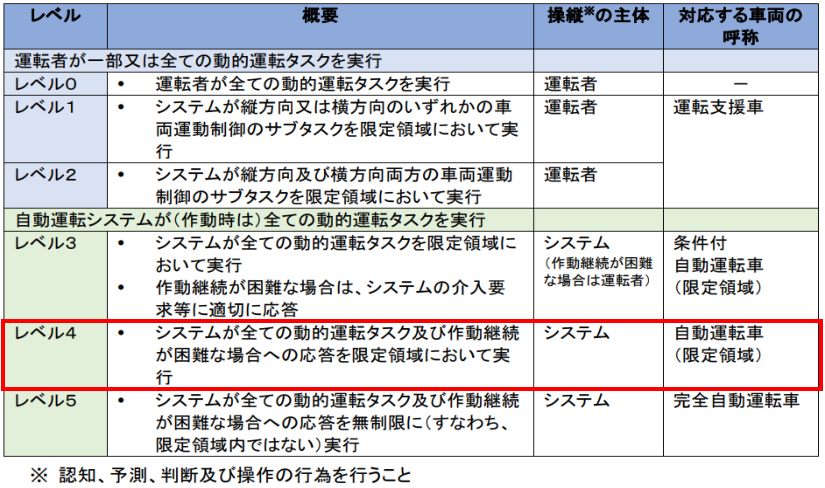
\includegraphics[width=.8\textwidth]{img/auto.pdf}
    \end{minipage}
  \end{figure}
{\tiny [参考] 官民ITS構想・ロードマップ2021 \url{https://cio.go.jp/sites/default/files/uploads/documents/its_roadmap_20210615.pdf}}
\end{frame}

\begin{frame}
  \frametitle{付録:研究事例}
  $\blacksquare$ ソフトウェアシミュレーション環境を利用した研究(実証実験)が多数存在\\
  \hrulefill\\
  \begin{itemize}
    \item 遠隔型自動運転システムにおける遠隔操作時の映像遅延が操舵に与える影響の評価${}^\text{1}$
    \item 自動車の遠隔操縦者の運転特性に関する研究(第一報) ${}^\text{2}$
    \item 自動運転車への信頼感向上のための自動運転シミュレータによる高運転パフォーマンス体験のもたらす効果${}^\text{3}$
  \end{itemize}
  \hrulefill\\
  \begin{center}
  \begin{minipage}{.5\linewidth}
    \begin{alertblock}{}
        \centering
        \Large \emph{\textcolor{red}{これらは全てシミュレーション上の\\実証実験環境}}
    \end{alertblock}
  \end{minipage}
\end{center}

  {\tiny [1] 水島知央, 神蔵貴久と大前学, 「遠隔型自動運転システムにおける遠隔操作時の映像遅延が操舵の操作に与える影響の評価」, 自動車技術会論文集, vol. 50, no. 3, pp. 970–976, 2019.}\\
  \vspace{-2.5truemm}
  {\tiny [2] 杉町敏之, 郭鐘聲と須田義大, 「自動車の遠隔操縦者の運転特性に関する研究（第一報）」, 生産研究, vol. 72, no. 2, pp. 191–194, 2020.}\\
  \vspace{-2.5truemm}
  {\tiny [3] 福田遼, 山本景子, 倉本到と辻野嘉宏, 「自動運転車への信頼感向上のための自動運転シミュレータによる高運転パフォーマンス体験のもたらす効果」,}\\
  \vspace{-2.5truemm}
  {\tiny ヒューマンコンピュータインタラクション（HCI）, vol. 2018-HCI-177, no. 11, pp. 1–8, 2018.}
\end{frame}

\begin{frame}
  \frametitle{付録:自動運転に関する動向}
  \centering
  \begin{minipage}{.8\linewidth}
    \begin{block}{自動運転の需要}
    地方都市圏への交通手段として注目(バス・タクシー等のラストワンマイル運転)
    \end{block}
    
    \begin{alertblock}{自動運転の課題}
      \begin{itemize}
        \item 自動運転の高度化$=$運転責任はシステムに移譲
        \begin{description}[ex.]
          \item[ex.] 自動運転レベル3：運行設計領域(ODD)で全ての運転を自動化
        \end{description}
        \begin{itemize}
          \item \textcolor{red}{システム要請により手動運転に戻る義務あり} → 運転責任がドライバに戻る
        \end{itemize}
        \item ドライバの自動手動切り替え対応の難しさ
      \end{itemize}
    \end{alertblock}
    \begin{exampleblock}{一例：遠隔型自動運転(自動運転レベル3以上)}
      \begin{itemize}
        \item 自動運転システムの異常時に遠隔操縦に切り替え
        \begin{itemize}
          \item ドライバーが遠隔地から車側のリアルタイム映像を見ながら操縦
        \end{itemize}        
        \item 自動運転の補助操作でも\textcolor{red}{免許と法定の訓練が必須}かつ\textcolor{red}{複数人での管理が必須}
      \end{itemize}
    \end{exampleblock}
  \end{minipage}
\end{frame}

\begin{frame}
  \frametitle{付録:卒業研究について}
  \centering
  \begin{minipage}{.8\linewidth}
    \begin{block}{免許・法定の訓練が不要な遠隔型自動運転システムの開発}
      \begin{description}[目的]
        \item[目的] 遠隔型自動運転の実験・練習及び研究のための運転環境構築
        \item[方法] 運転免許未所持者に対する操作\textcolor{red}{確度}の解析(\textcolor{red}{インターフェース}と\textcolor{red}{走行環境}を比較)
      \end{description}
    \end{block}
    \begin{exampleblock}{成果}
        \begin{itemize}
          \item 速さ → \textcolor{red}{ゲームパッド}$>$ステアリングコントローラ (コース走行タイム\textcolor{red}{12 \% }優)
          \item 安全性 → \textcolor{red}{ステアリングコントローラ}$>$他2つ(壁面への接触\textcolor{red}{47.5 \% }少)\\
          ステアリングコントローラ$=$\textcolor{red}{安全かつ習熟度が最も高い}
        \end{itemize}
    \end{exampleblock}
    \begin{alertblock}{結論}
      \begin{itemize}
        \item \textcolor{red}{ステアリングコントローラ}が運転用インターフェースとして最適
      \end{itemize}
    \end{alertblock}
  \end{minipage}
\end{frame}

\begin{frame}
  \frametitle{付録:卒業研究とのつながり}
  \centering
  \begin{minipage}{.8\linewidth}
    \begin{block}{課題}
      ステアリングコントローラが運転用インターフェースとして最適であるが...
      \begin{itemize}
        \item 実車と比べて\textcolor{red}{簡単} → \textcolor{red}{操作の難易度が相対的に上がると？}
        \begin{description}[ex.1]
          \item[ex.1] 幅広い運転技能を持つ被験者に対する検証(20代のみ → 未就学児～高齢者)
          \item[ex.2] ユーザインターフェースMTやセミオートマ等の操作環境では？
        \end{description}
      \end{itemize}
    \end{block}

    \begin{alertblock}{目標設定}
      \begin{description}[目的]
        \item[目的] インターフェースの操作性に基づく運転技能解析の追究
        \item[提案] ROSを用いた遠隔型自動運転システム
        \item[方法] MTインターフェースによる遠隔型自動運転の操作性解析環境
      \end{description}
    \end{alertblock}
  \end{minipage}
\end{frame}

\begin{frame}
  \frametitle{付録: ROSについて}
  $\blacksquare$ ロボットソフトウェアプラットフォーム\\
  $\blacksquare$ ROSを用いるメリット
  \begin{itemize}
    \item ロボット用アプリケーションプログラムの開発に必要なライブラリ開発環境が豊富
    \begin{itemize}
      \item 位置推定/地図作成(SLAM)/ナビゲーション用のライブラリツール群
    \end{itemize}
    \item 分散プロセス
    \begin{itemize}
      \item 最小実行単位(ノード)のプロセスで全体機能が実現
      \item 各ノードが独立して並列的に動作
      \item 双方向のデータ送受信が可能
    \end{itemize}
    \item パッケージ管理
    \begin{itemize}
      \item 同一の目的で作成された複数のノードはまとめてパッケージとして管理
    \end{itemize}
  \end{itemize}
\end{frame}

\begin{frame}
  \frametitle{付録:システム構成}
  \begin{figure}
    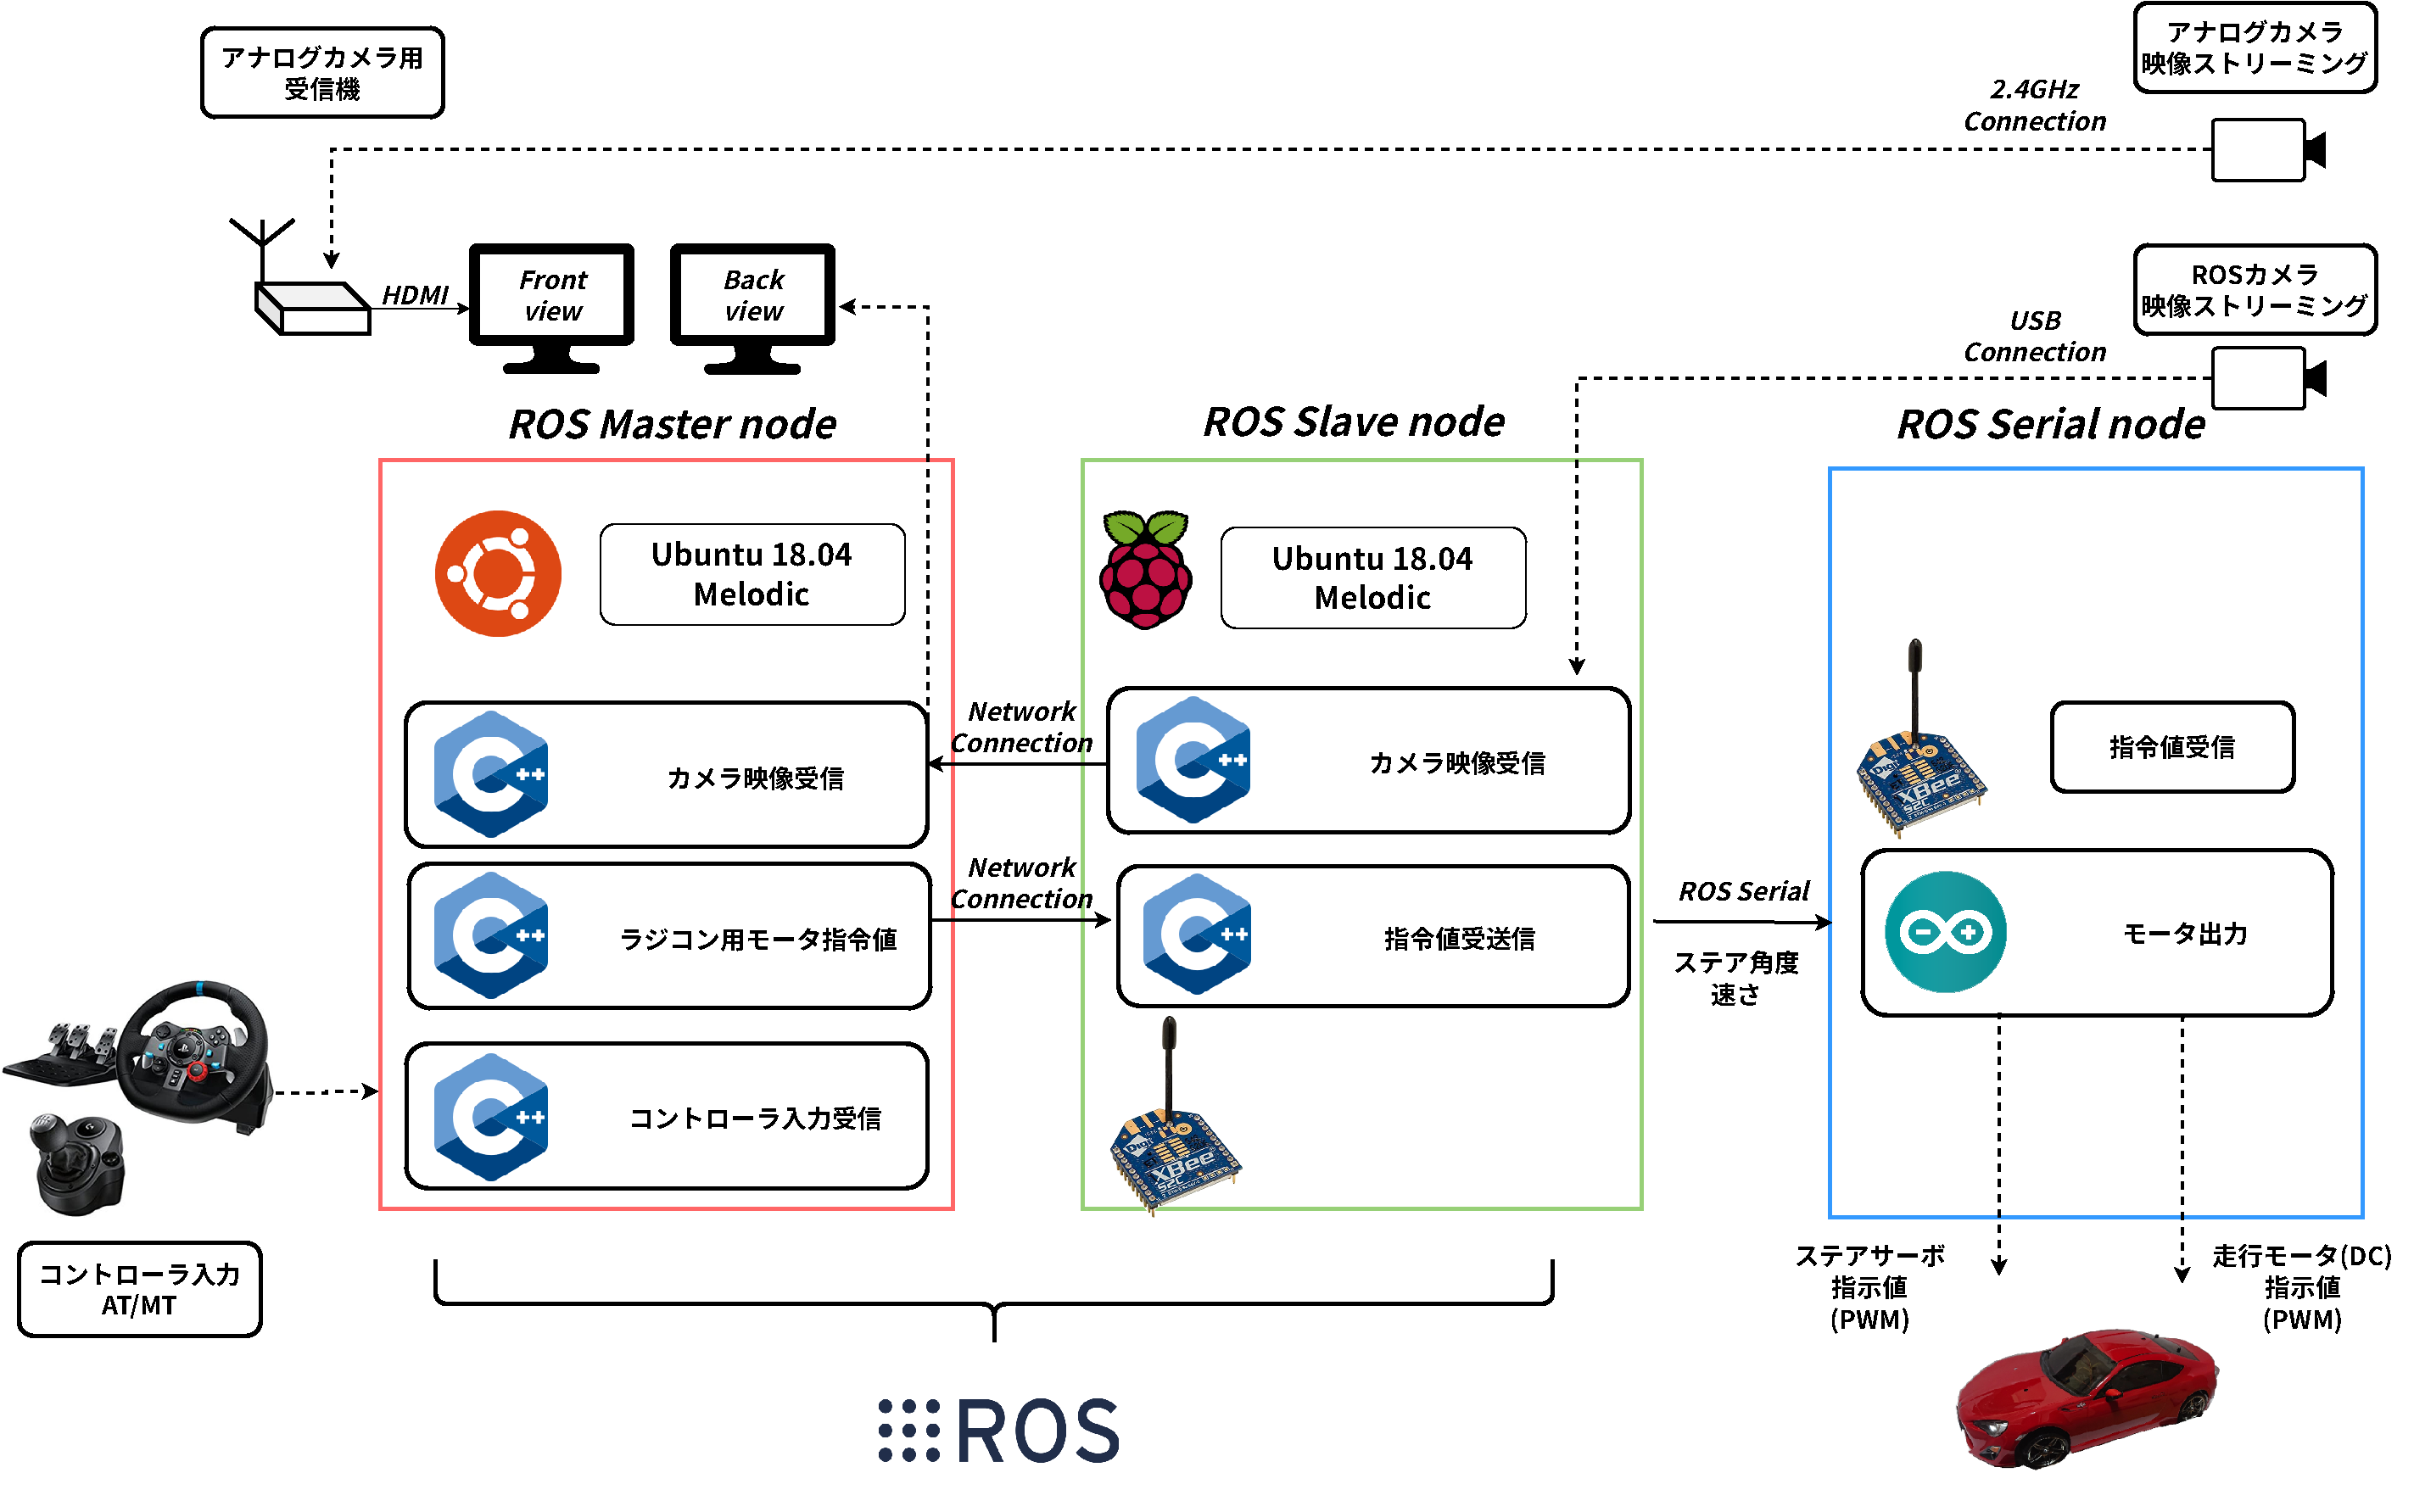
\includegraphics[width=.8\textwidth]{img/previous_struct.pdf}
  \end{figure}
\end{frame}

\begin{frame}
  \frametitle{付録:使用機器}
  \centering
  \begin{tabular}{llll}
    \noalign{\hrule height 1pt}
    使用機器　 & 製品名 \\
    \hline
    RCカー & TAMIYA 1/10XBシリーズ TOYOTA86 \\
    ステアリングコントローラ & Logicool G27 Steering Wheel \\
    シフトレバー & Logicool Driving Force Shifter \\
    マスターPC & Lenovo Thinkpad X230 \\
    スレーブPC & Raspberry Pi 4 Model B 4GB \\
    OS & Ubuntu 18.04 LTS \\
    ミドルウェア & ROS Melodic \\
    マイコン & Arduino Uno R3 \\
    通信モジュール & Xbee S2C \\
    フロントカメラ & AKK S2 FPVカメラ 600TVL\\
    バックカメラ & Logicool C270n\\
    \noalign{\hrule height 1pt}
    \end{tabular}    
\end{frame}

\begin{frame}
  \frametitle{付録:体感速度に関して}
  $\blacksquare$ 本システムの実速度をスケール換算した速度を体感速度としている。
  \begin{itemize}
    \item フルード数の計算方法より、$1/10$スケールの場合、実速度を$\sqrt{10}$ 倍した値を体感速度としている。
  \end{itemize}
    \vspace{-8pt}

    \hrulefill

    \begin{center}
      \begin{minipage}{.8\linewidth}
          \begin{block}{}
              \centering
              \begin{tabular}{cc}
                \small ピクセルの移動距離と実距離について\\
                  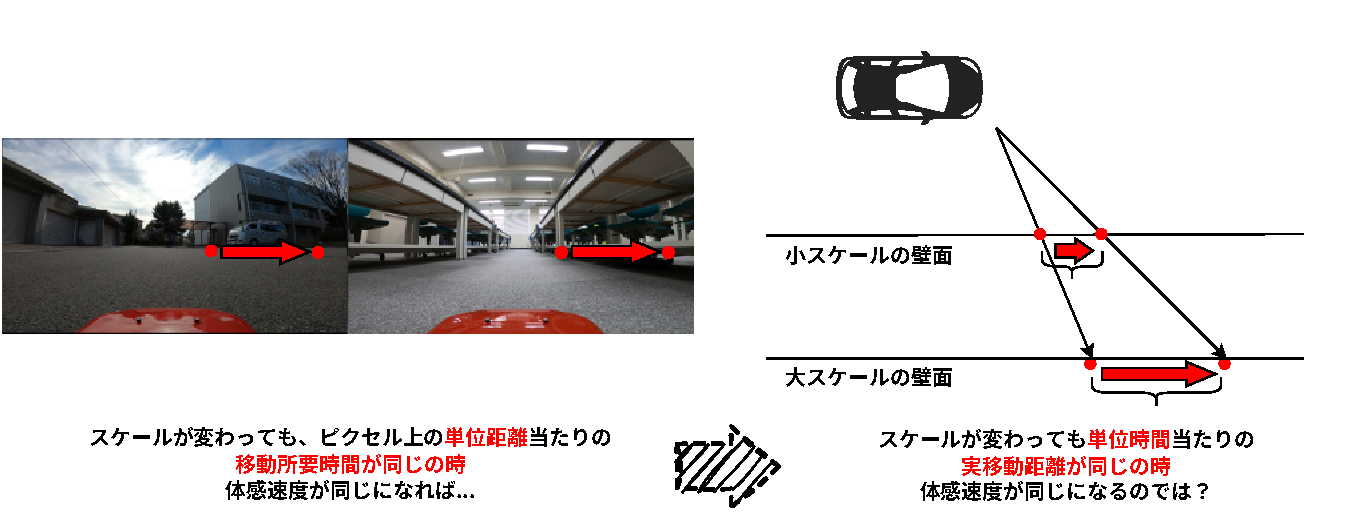
\includegraphics[height=.4\textheight]{img/taikan2.pdf}
              \end{tabular}
          \end{block}
      \end{minipage}
  \end{center}
\end{frame}

% \begin{frame}
%   \frametitle{video}
%   \includemedia[
%     activate=pageopen,
%     width=140pt,height=100pt,
%     addresource=./ope1.mp4,
%     flashvars={%
%        src=hoge.mp4%
%        &autoPlay=false%
%        &scaleMode=stretch%
%        &volume=0%
%        &loop=true%
%     }  
%   ]{}{StrobeMediaPlayback.swf}
% \end{frame}

\begin{frame}
  \frametitle{付録:走行実験の様子}
\end{frame}

\end{document}